\chapter{Python}
\begin{figure}[h]
    \centering
    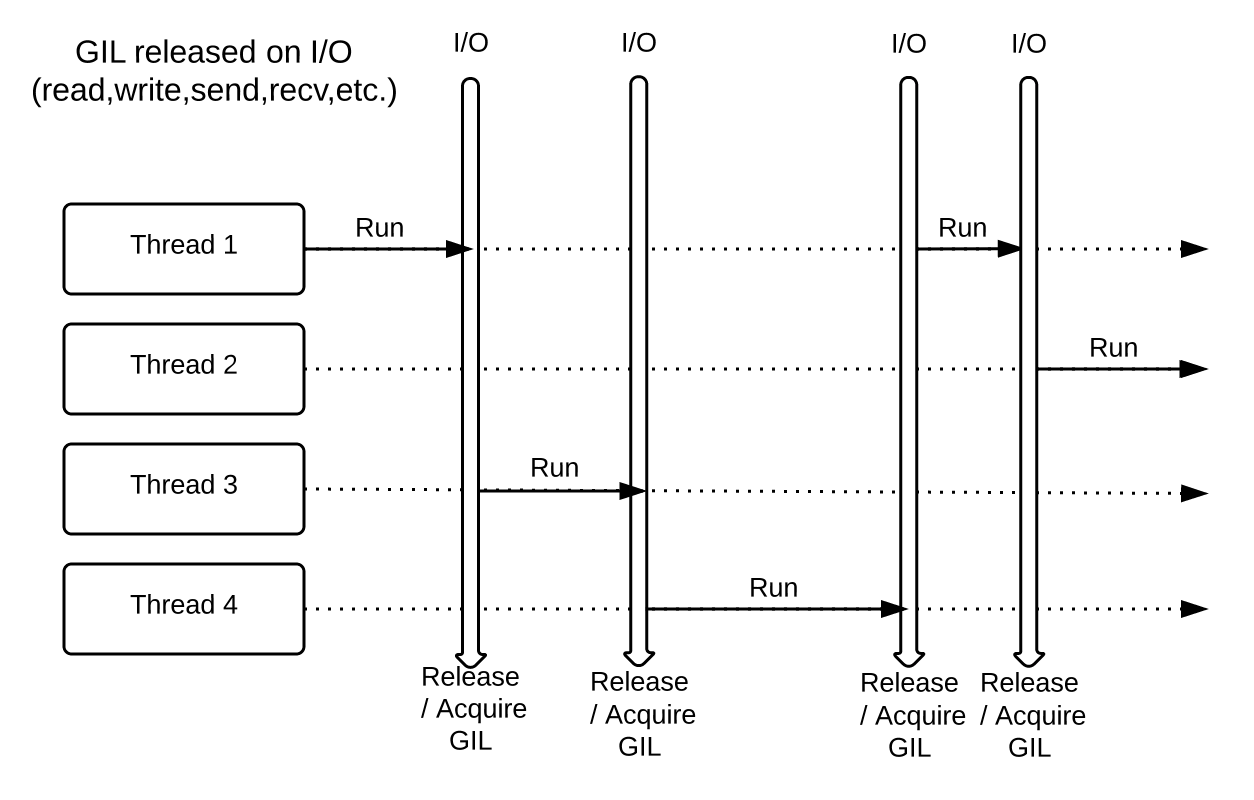
\includegraphics[scale=0.5]{images/GIL.png}
    \caption{Fonctionnement du Global Interpreter Lock.}
    Les programmes IO bound (avec beaucoup d'entrées-sorties) ne sont pas limités par le GIL. Leurs demandes sont envoyées au système d'exploitation qui les traîte ensuite. En revanche les threads des programmes CPU bound ("beaucoup d'instructions à executer") tournent un par un. Ce qui est contre-intuitif lorsqu'on parle de mutli-threading.\footnote{http://www.dabeaz.com/python/UnderstandingGIL.pdf}.
\end{figure}

\chapter{Miasm}
\begin{figure}[h]
    \centering
    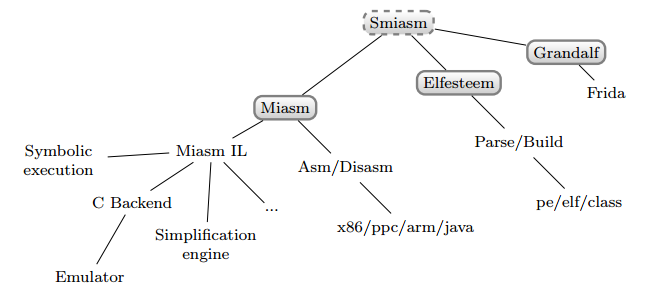
\includegraphics[scale=0.5]{images/miasm-orga.png}
    \caption{Composants de miasm.}
    Architecture de l'outil Miasm\footnote{https://www.sstic.org/media/SSTIC2012/SSTIC-actes/miasm\_framework\_de\_reverse\_engineering/SSTIC2012-Article-miasm\_framework\_de\_reverse\_engineering-desclaux\_1.pdf}.
\end{figure}
